%% GroveFS — ACM Transactions on Storage (TOS) long-form manuscript.
%% Formal-model + correctness-proof chapter (Sec. 5) written to be compilable.
%%
%% Build: needs TeX Live with the `acmart` class (acmtos option).
%%   tlmgr install acmart          # if missing
%%   latexmk -pdf grovefs-tos.tex  # pdflatex xelatex both fine
%%
%% NOTE: this source has been machine-compiled with TeX Live (latexmk/pdfLaTeX,
%% 20 pages, no errors) including the Sec. 6 agent-MCP/API-key paragraph, the
%% Sec. 7 executed mcp/apikey evidence and the Sec. 8 agent-interface
%% positioning. Re-run `latexmk -pdf grovefs-tos.tex` after any edit.

\documentclass[numberedsection,acmtos]{acmart}

\usepackage{tikz}
\usepackage{enumitem}
\usetikzlibrary{arrows.meta,positioning,fit,backgrounds}

%% ---------------------------------------------------------------- metadata
\setcopyright{acmcopyright}
\copyrightyear{2026}
\acmYear{2026}
\acmDOI{}
\acmJournal{TOS}
\acmVolume{0}
\acmNumber{0}
\acmArticle{0}
\acmMonth{0}

\begin{document}

\title[GroveFS]{GroveFS: Identity-Preserving, Centrally-Governed Views over a
Single Authoritative Namespace}

\author{Anonymous Author(s)}
\affiliation{%
  \institution{Anonymous Institution}
  \country{Anonymous}}
\email{anon@example.org}

\renewcommand{\shortauthors}{Anonymous et al.}

\begin{abstract}
Next-generation astronomical surveys hand science platforms petabyte-to-exabyte
archives that many users must browse and analyse without the data being copied
onto user-facing storage. This is an instance of a control-plane question that
current systems treat as an afterthought: who sees which shape of the same
authoritative data, under which name, and how are those decisions governed
centrally without breaking identity. Subtree mounts, overlayfs, symbolic links
and bind mounts with ACLs each solve part of the problem, but none keeps a
single body of bytes tied to exactly one real inode while the namespace over it
is reshaped, aliased, rotated and onboarded under central governance. We show
that performing this reshaping inside the metadata layer, as a source-path
translation that never duplicates directory entries, makes four capabilities
available at once that otherwise conflict: server-side read-only derived views,
atomically rotatable aliases, per-client display lenses, and zero-copy import of
legacy data. We formalise the model, state four invariants (I1--I4) and prove
them, and evaluate the design on expressiveness and correctness, including a
counterexample study against hand-composed overlay, symlink, bind and ACL
stacks. The embedded single-writer backend carries no throughput or scalability
claim. On the PostgreSQL backend we adopt the HopsFS approach of per-operation
SERIALIZABLE transactions under PostgreSQL SSI with bounded retry; the
invariants carry over unchanged to any serialisable schedule, replacing the
single physical writer with its serial-equivalence class without weakening the
governance result.
\end{abstract}

\begin{CCSXML}
<ccs2012>
<concept><concept_id>10003033.10003079</concept_id>
<concept_desc>Storage design</concept_desc><concept_significance>500</concept_significance></concept>
<concept><concept_id>10003456.10003462.10003464</concept_id>
<concept_desc>Software and its engineering~File systems</concept_desc><concept_significance>500</concept_significance></concept>
</ccs2012>
\end{CCSXML}
\ccsdesc[500]{Storage design}
\ccsdesc[300]{Software and its engineering~File systems}

\keywords{namespace governance, multi-tenancy, FUSE, view composition,
zero-copy import, correctness proofs}

\maketitle

%% ================================================================= 1-4 stubs
\section{Introduction}
\label{sec:intro}
A concrete driver of this work is data-intensive astronomy. Next-generation
telescopes and surveys produce petabyte-to-exabyte archives, and the science
platforms serving them must let many users browse and analyse the data without
it being copied onto login or analysis nodes. The archive stays a single
authoritative store, while each consumer sees a governed view of it, such as a
public data release, an instrument- or programme-restricted subset, or a
reorganised projection, rather than a fresh clone \citep{han2026yourfs}. The
same problem recurs wherever shared storage is multi-tenant: one body of
authoritative data is consumed by many users, roles and services that each need
a different presentation of it. A research group wants a dataset shown only as
the documents it contains; a compliance officer wants the same files reached
under a public name that can be withdrawn the moment it leaks; an operator wants
a legacy tree already sitting on disk to join the namespace without moving a
byte. These are facets of a single control-plane problem, spanning visibility,
naming, shape and onboarding, posed over one authoritative namespace.

Existing systems address parts of this problem but treat it as an afterthought.
Distributed and parallel filesystems such as CephFS, Lustre and GPFS expose
tenancy as a fixed subtree: a client mounts a path, and any other shape is
obtained by gluing primitives, such as bind mounts, symbolic links, overlay
layers and POSIX ACLs, on top. Each glue is fine in isolation, yet none is
centrally governed, in that the reshaping lives in per-client configuration
rather than in the authority that owns the data, and combining them breaks
identity. Overlayfs copies a file into a distinct upper object on first write,
so the bytes exist in two divergent bodies; a symbolic link materialises an
extra entry that dangles once its target is removed; and a bind mount equates
the mount path with the storage identity, so a public name cannot be rotated
without exposing the real one.

Our position is that view governance deserves to be a first-class,
identity-preserving concern. We state four invariants (I1--I4,
Sec.~\ref{sec:inv}) capturing that a single body of bytes must retain exactly
one real inode while the namespace over it is reshaped, aliased, rotated and
onboarded, and we show that if the reshaping is performed in the metadata layer
as a source-path translation that never duplicates directory entries, then four
capabilities that otherwise conflict become simultaneously expressible and
provably correct: server-side derived read-only views, atomically rotatable
aliases, per-client display lenses, and zero-copy onboarding of legacy data.
The design is orthogonal to, and composable with, data-placement and
concurrency mechanisms.

This paper makes the following contributions.
\begin{itemize}
  \item A model of centrally-governed, identity-preserving views built on
        the classical inode/dentry store (Sec.~\ref{sec:model}) and four
        invariants I1--I4 that
        separate genuine view governance from the glue of hand-composed
        primitives.
  \item An invariant-based correctness argument: two lemmas (no
        aliasing collision, derived non-forking) and a proof sketch of a
        main theorem that a well-formed composition of the
        primitives preserves I1--I4 (Sec.~\ref{sec:formal}). The lens-level
        invariants I1, I2 and I4 are additionally checked by execution, via a
        randomised property test that drives the real implementation over
        hundreds of seeded (tree, rule-set) compositions (Sec.~\ref{sec:formal},
        Sec.~\ref{sec:eval}).
  \item Four orthogonal governance primitives realised over a single
        authoritative metadata service and, transparently, over both an
        embedded and a PostgreSQL metadata backend.
  \item An executable falsification of the alternative: a self-contained
        harness (the \texttt{govcheck} and \texttt{govtime} suites) that
        reproduces where overlay, symlink, bind and ACL stacks violate I1--I4
        and shows GroveFS satisfies the same assertions, with measured
        control-plane convergence windows (Sec.~\ref{sec:eval}).
\end{itemize}

\paragraph{Scope.}
This is a control-plane contribution. We make no throughput or scalability
claim: the metadata service serialises writes on a single authoritative writer,
with reads fanning out over a bounded pool. Sec.~\ref{sec:limits} and
Sec.~\ref{sec:discussion} state this boundary precisely.

\section{Problem Statement and Governance Primitives}
\label{sec:problem}

\paragraph{A running example.}
Throughout we use one authoritative tree, view \emph{team}, holding
\texttt{/docs/2026/report.md}, \texttt{/photos/private/x.jpg},
\texttt{/photos/public/y.jpg} and \texttt{/data/raw/big.bin}. Three consumers
share it: an analyst who should see only documents, a public portal that must
show \texttt{/data/raw} under a friendly path and never reveal the private
album, and an auditor who reaches the whole tree through a public name that can
be recalled if it leaks. We show each need is a \emph{distinct primitive} and
that they compose over the one stored tree.

\paragraph{Astronomy instantiation.}
The same three consumers appear on a survey platform \citep{han2026yourfs}.
The authoritative tree is a science/calibration archive; the analyst is a
proposing team restricted to their own programme's pointings; the public portal is
a data-release view that re-homes raw products under a friendly hierarchy and must
never reveal embargoed frames; the auditor is a transient public alias for a
release that has to be revocable the instant an embargo is breached. None of
this may be served by cloning the archive onto user-facing storage, the
non-landing requirement, which is exactly the identity-preserving,
centrally-governed view this paper provides. The generic running example above is
this scenario stripped of its domain names.

\paragraph{Governance dimensions.}
We decompose view governance along four axes, each exercised by the running
example:
\begin{itemize}
  \item Visibility: which subtrees a mount may see at all. The analyst hides
        everything but documents; the portal masks the private album. This is
        realised by the display lens (\texttt{hide}, \texttt{only}).
  \item Shape: how visible entries are arranged. The portal
        re-homes \texttt{/data/raw} to \texttt{/team/raw} without moving bytes.
        This is realised by \texttt{map}/\texttt{link} and, when centrally
        managed, by server-side derived views.
  \item Naming: what the entry point is called, and whether that
        name can be rotated. The auditor's public alias is a governance handle
        separable from the storage identity.
  \item Onboarding: how pre-existing bytes join the namespace. A
        legacy directory already on disk should appear in a view without being
        copied.
\end{itemize}

\paragraph{Why existing mechanisms fall short.}
No single existing mechanism spans these dimensions while preserving identity.
A fixed subtree mount gets visibility but not cross-parent shape or rotation.
Symlinks reach an entry from a second location, but they add a separate
directory entry, dangle when the target is deleted, and expose the concrete
storage path, defeating naming governance. Overlayfs reorganises by copying on
write, forking one object into two divergent bodies. Bind mounts with ACLs scope
a fixed subtree and make the mount path the secret. The difficulty is
structural: each of these either duplicates the entry or moves the bytes, and
identity preservation forbids both.

\paragraph{The required invariant.}
We therefore require that reshaping be a pure presentation over one stored
tree: the bytes keep exactly one real inode, and reference counting,
reclamation, locking and cross-client invalidation all remain keyed on it.
Sec.~\ref{sec:formal} states this as four invariants (I1 entry uniqueness, I2
identity-preserving sharing, reclamation and locking, I3 invalidation integrity,
I4 write-through to source) and proves the primitives satisfy them.

\paragraph{The primitives.}
GroveFS realises the dimensions above as four orthogonal, composable primitives
over a single authoritative namespace: the display lens (per-mount, client-side
rules), the derived view (the same lens rules but centrally defined and
server-rendered, read-only), the alias (pure name governance with atomic
rotation), and import (zero-copy onboarding). They compose: an imported tree
can be a relocation source, a derived view can be layered over an alias, and a
per-mount lens sits above any metadata backend. A fifth, complementary
primitive---the fork view---provides an organisation sandbox that copies
namespace rows while sharing bytes; it is presented separately because it
deliberately lies outside the translation core. A sixth mechanism, per-view
metadata export and import (Sec.~\ref{sec:portability}), is orthogonal in kind:
it \emph{moves} a tree between stores instead of reshaping it, and it is
possible at all because the row format carries no location.

\section{Design Overview}
\label{sec:design}
GroveFS is a userspace (FUSE) filesystem factored along two trait seams so that
governance is a presentation concern independent of where bytes and
tree-structure physically live.

\paragraph{Layers.} The FUSE mount process sits above a
\texttt{MetaProvider} trait (view-tree access: lookup, getattr, readdir,
create, rename, unlink, setattr, lock) and a \texttt{StorageBackend} trait
(object IO). Local engines store one SQLite database per view and objects
under \texttt{blocks/}, fanned out over 256 hash-bucketed subdirectories so
no single directory grows with the object count (tens of millions of objects
keep per-directory entry counts, and with them backup and traversal cost,
bounded); the placement is a pure function of the object key, so metadata
pointers are unaware of it. Remote clients talk over a custom framed TCP protocol
to a central \texttt{meta-server} and \texttt{data-server}; a sharded backend
stripes objects across several data-servers. The authoritative metadata store
is either the embedded engine or PostgreSQL (schema-per-view, transactional
rename/unlink/lock), transparently to clients.

\paragraph{Where governance lives.} The view primitives are decorations of
\texttt{MetaProvider}: the lens wraps any provider, local or remote, and
translates display paths to source paths below the FUSE layer and above the
authority. This placement matters. Because translation happens at the metadata
interface rather than in a kernel union layer, the lens never materialises an
entry: a relocated or aliased display name resolves to the one existing
directory row, so all writes, reference counts, garbage collection, advisory
locks and invalidation events pass through to the source inode. Governance is
thus a read-through projection, not a second copy of state.

\paragraph{Authority and consistency.} Governance lives above a single
authoritative metadata store, but that store takes one of two shapes. Under the
embedded engine (one SQLite database per view) a view's tree is mutated by
exactly one writer connection, which is what makes I3 and the lock arbitration
of Sec.~\ref{sec:formal} well-defined. Under the PostgreSQL backend, in the
spirit of HopsFS \citep{hopsfs}, the store admits concurrent writers: each
mutating operation runs as its own \texttt{SERIALIZABLE} transaction checked out
from a bounded writer pool, PostgreSQL SSI \citep{ports2012} detects read--write
dependency cycles and aborts one side with \texttt{SQLSTATE\,40001}, and the
client retries with bounded exponential backoff. Reads fan out over a separate
pool. Because every accepted schedule is serialisable, it is equivalent to some
run of a single authoritative writer, so I1--I4 carry over from the serial case
and neither the invalidation events nor the lock table need a global physical
ordering. After a successful write the server pushes
\texttt{inval\_entry} and \texttt{inval\_inode} events to the view's other
subscribers, referencing source inodes, so a peer's change is visible on the
next lookup without polling; a zero-cache strict mode is offered as a fallback.

\paragraph{Access control.} Authority over a tree is separated from the
governance layer that shapes it, and is exercised entirely on the open handshake
of both planes (\texttt{meta-server} \texttt{M\_OPEN}, \texttt{data-server}
\texttt{OP\_OPEN}). A shared cluster token admits a host to the whole store (an
empty token is LAN-trusted); optionally a per-caller API key, required by
\texttt{--require-api-key} and kept only as SHA-256 digests in a local
control-plane SQLite registry, replaces that coarse gate with revocable,
auditable credentials. Each key then carries two orthogonal access dimensions
in place of any per-user permission table: \texttt{--view} binds it to a single
physical view (checked after alias resolution, so a grant written for the real
name still holds through a rotated alias), and \texttt{--ro} makes it read-only,
every write-intent operation---advisory locks included---refused at the
authoritative per-op gate even against a client that mounted writable. The
outcome codes stay distinct from data faults: admission failure is
\texttt{E\_AUTH}, a read-only key's write is \texttt{E\_NOTPERM} (\texttt{EPERM}
at FUSE, content writes \texttt{EROFS}), and the standby's failover signal
\texttt{E\_ROFS} is kept apart so a client fails over rather than reading it as
a denial. Crucially the presenting \texttt{uid} never gates access: it is
advisory (a TCP client can spoof it), recorded only as the lock/audit owner via
\texttt{geteuid()} or an \texttt{--as-uid} override. Display lenses and derived
views are customisation, not a security boundary; hard isolation is always the
view plus its token or key.

\paragraph{Orthogonality.} Placement, striping, replication/HA and concurrency
are separate concerns the governance layer neither assumes nor forecloses; the
primitives compose over any backend and over a shared server, and are
orthogonal to the data-plane mechanisms other systems (e.g.\ SplitFS)
optimise.

\begin{figure}[t]
\centering
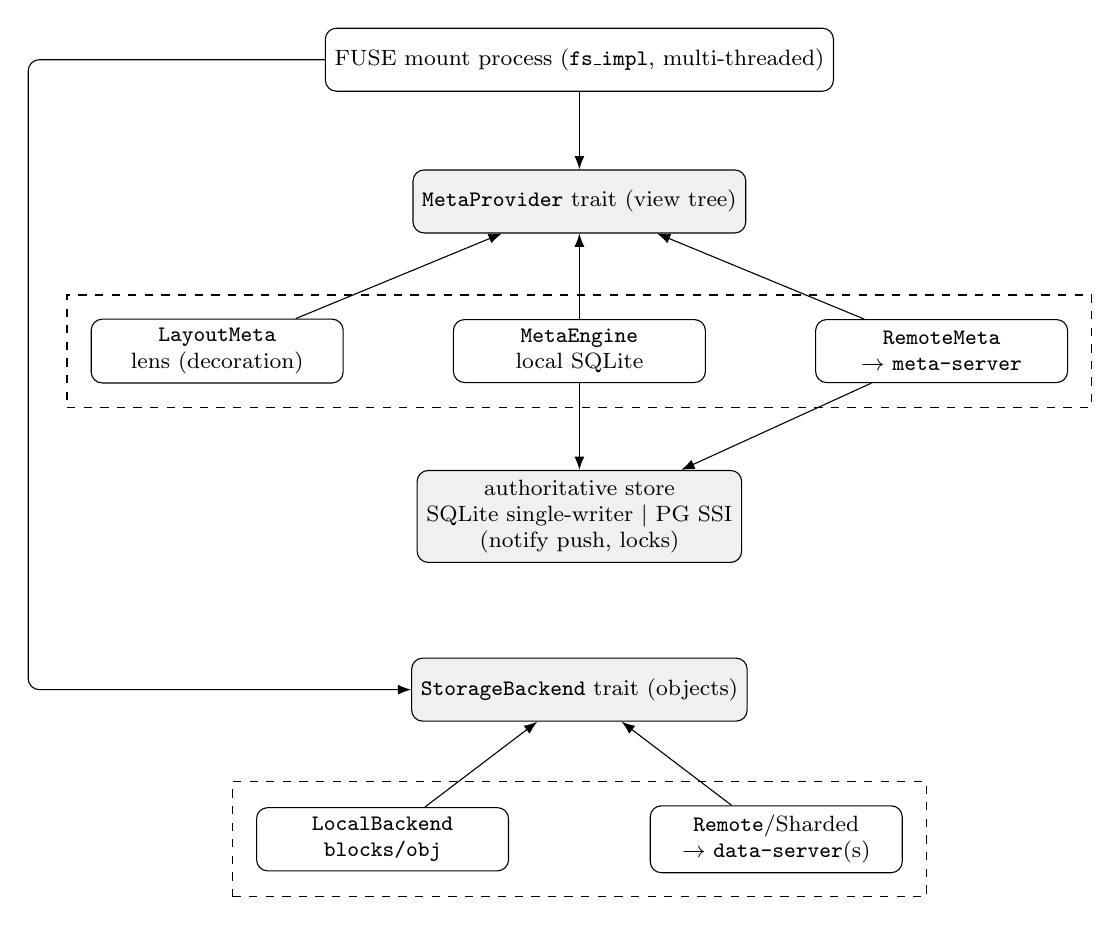
\begin{tikzpicture}[
  box/.style={draw,rounded corners,align=center,minimum height=8mm,font=\footnotesize},
  trait/.style={box,fill=black!6},
  imp/.style={box,minimum width=32mm}]
\node[box] (fuse) at (0,0) {FUSE mount process (\texttt{fs\_impl}, multi-threaded)};
\node[trait] (meta) at (0,-1.8) {\texttt{MetaProvider} trait (view tree)};
\node[imp] (lens) at (-4.6,-3.7) {\texttt{LayoutMeta}\\ lens (decoration)};
\node[imp] (loc)  at (0,-3.7) {\texttt{MetaEngine}\\ local SQLite};
\node[imp] (rem)  at (4.6,-3.7) {\texttt{RemoteMeta}\\ $\to$ \texttt{meta-server}};
\node[trait] (auth) at (0,-5.8) {authoritative store\\ SQLite single-writer $\mid$ PG SSI\\ (notify push, locks)};
\node[trait] (sto) at (0,-8.0) {\texttt{StorageBackend} trait (objects)};
\node[imp] (bloc)   at (-2.5,-9.9) {\texttt{LocalBackend}\\ \texttt{blocks/obj}};
\node[imp] (bshard) at (2.5,-9.9) {\texttt{Remote}/{Sharded}\\ $\to$ \texttt{data-server}(s)};
% control plane: FUSE drives the metadata trait; implementations funnel writes
\draw[-{Latex}] (fuse) -- (meta);
\draw[-{Latex}] (lens) -- (meta);
\draw[-{Latex}] (loc) -- (meta);
\draw[-{Latex}] (rem) -- (meta);
\draw[-{Latex}] (loc) -- (auth);
\draw[-{Latex}] (rem) -- (auth);
% data plane: FUSE reaches the object store directly (side lane), orthogonal to
% the metadata seam -- drawn outside the boxes so it crosses nothing
\draw[-{Latex},rounded corners] (fuse.west) -- (-7,0) -- (-7,-8.0) -- (sto.west);
\draw[-{Latex}] (bloc) -- (sto);
\draw[-{Latex}] (bshard) -- (sto);
\begin{scope}[on background layer]
\node[draw,dashed,fit=(lens)(loc)(rem),inner sep=3mm] {};
\node[draw,dashed,fit=(bloc)(bshard),inner sep=3mm] {};
\end{scope}
\end{tikzpicture}
\caption{GroveFS layering. Governance (lens, derived views, aliases) decorates
the \texttt{MetaProvider} seam and is transparent to the FUSE layer and
orthogonal to the \texttt{StorageBackend} seam; all providers funnel writes into
one authoritative store (either a single-writer connection, or a serialisable
pool of writers under PostgreSQL SSI).}
\label{fig:arch}
\end{figure}

\section{Mechanisms}
\label{sec:mechanisms}

\subsection{The Display Lens (visibility and shape, per mount)}\label{sec:lens}
A mount may pass \texttt{--layout rules.txt} to wrap its provider with a
translation lens (Fig.~\ref{fig:lens}). Rules are plain text, one verb per line, evaluated against
\emph{source} paths: \texttt{hide \textless src\textgreater} drops a subtree; \texttt{only \textless src\textgreater}
whitelists (showing only these subtrees plus the ancestors needed to reach
them); \texttt{map \textless src\textgreater{} \textless dst\textgreater{}} re-homes an entry to \texttt{\textless dst\textgreater{}} and vacates
its source spot; \texttt{link \textless src\textgreater{} \textless dst\textgreater{}} shows it at \texttt{\textless dst\textgreater{}} \emph{and}
keeps the source spot, the two names sharing one real inode. Filters and
relocations compose without contradiction: \texttt{map}/\texttt{link} display a
subtree regardless of a filter at the source spot, while filtering still
applies \emph{inside} the moved subtree by source path.

Intermediate display directories that exist in no source view are synthesised
from a reserved high inode range and are never persisted; creating directly
inside one is refused with \texttt{EPERM} (there is no source anchor). A
\texttt{map} leaf overrides the reported name and parent so that \texttt{..}
and attributes stay inside the lens; a \texttt{link} alias keeps its canonical
source identity, and its \texttt{..} leads to the source parent. Path-to-inode
resolutions expire after a short TTL matching the kernel cache, and a local
mutation flushes them.

\begin{figure}[t]
\centering
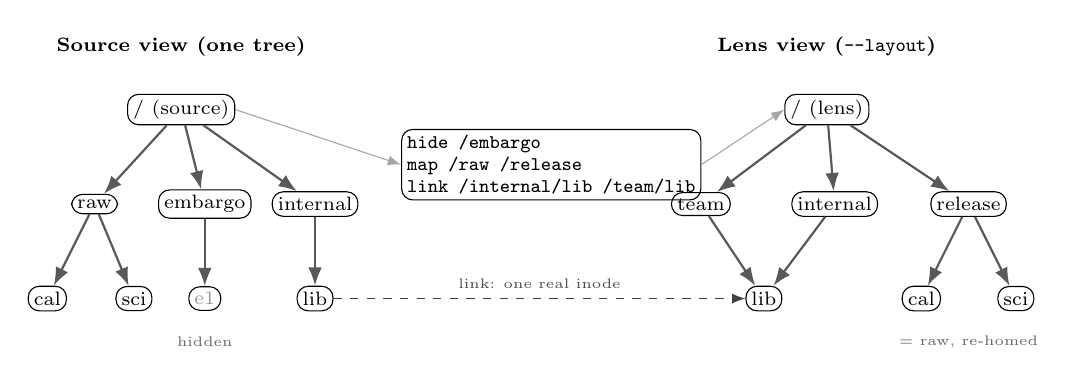
\begin{tikzpicture}[
  nn/.style={draw,rounded corners,inner sep=2pt,font=\scriptsize,align=center},
  dim/.style={nn,text=black!40},
  nt/.style={font=\tiny,text=black!60},
  ed/.style={-{Latex},draw=black!65,thick},
  sh/.style={-{Latex},dashed,draw=black!75}]
% source tree (left)
\node[font=\scriptsize\bfseries] at (1.4,6.1) {Source view (one tree)};
\node[nn] (sroot) at (1.4,5.3) {/ (source)};
\node[nn] (sraw)  at (0.3,4.1) {raw};
\node[nn] (semb)  at (1.7,4.1) {embargo};
\node[nn] (sint)  at (3.1,4.1) {internal};
\node[nn] (sr1)   at (-0.3,2.9) {cal};
\node[nn] (sr2)   at (0.8,2.9) {sci};
\node[dim] (se1)  at (1.7,2.9) {e1};
\node[nn] (slib)  at (3.1,2.9) {lib};
\draw[ed] (sroot)--(sraw); \draw[ed] (sroot)--(semb); \draw[ed] (sroot)--(sint);
\draw[ed] (sraw)--(sr1);  \draw[ed] (sraw)--(sr2);   \draw[ed] (semb)--(se1); \draw[ed] (sint)--(slib);
\node[nt] at (1.7,2.35) {hidden};
% rules (centre)
\node[nn,align=left] (rl) at (6.1,4.6) {\texttt{hide /embargo}\\\texttt{map /raw /release}\\\texttt{link /internal/lib /team/lib}};
\draw[draw=black!35,-{Latex}] (sroot.east) -- (rl.west);
% lens tree (right)
\node[font=\scriptsize\bfseries] at (9.6,6.1) {Lens view (\texttt{--layout})};
\node[nn] (lroot) at (9.6,5.3) {/ (lens)};
\node[nn] (lteam) at (8.0,4.1) {team};
\node[nn] (lint)  at (9.7,4.1) {internal};
\node[nn] (lrel)  at (11.4,4.1) {release};
\node[nn] (llib)  at (8.8,2.9) {lib};
\node[nn] (lr1)   at (10.8,2.9) {cal};
\node[nn] (lr2)   at (12.0,2.9) {sci};
\draw[ed] (lroot)--(lteam); \draw[ed] (lroot)--(lint); \draw[ed] (lroot)--(lrel);
\draw[ed] (lteam)--(llib);  \draw[ed] (lint)--(llib);  \draw[ed] (lrel)--(lr1); \draw[ed] (lrel)--(lr2);
\draw[draw=black!35,-{Latex}] (rl.east) -- (lroot.west);
\node[nt] at (11.4,2.35) {$=$ raw, re-homed};
% identity: the link alias shares the one real inode
\draw[sh] (slib) -- (llib) node[midway,above,font=\tiny,text=black!70] {link: one real inode};
\end{tikzpicture}
\caption{The display lens re-projects one authoritative source tree without
materialising a second copy. \texttt{embargo} is hidden; \texttt{raw} is
re-homed to \texttt{release} (same inodes, source spot vacated); and
\texttt{internal/lib} is aliased at \texttt{team/lib} while its source spot is
kept; the two display names resolve to one real inode (dashed).}
\label{fig:lens}
\end{figure}

\subsection{Server-Side Derived Views (centrally-governed shape)}
When shape must be managed by the authority rather than by each client, the
same rules are defined once with \texttt{view define --name \textless v\textgreater{} --base \textless b\textgreater{}}
\texttt{--rules F}, stored under \texttt{meta/views/\textless v\textgreater{}.layout} with a first line
\texttt{base \textless b\textgreater{}}; clients mount \texttt{--view \textless v\textgreater{}} with \emph{no local rule
file}. A derived view is a read-only projection enforced on two independent
layers: the open handshake flags the derived name so the kernel mount is
read-only (writes return \texttt{EROFS}), and the metadata service refuses
write-intent operations addressed to the derived name even against a
malformed client. Writes therefore belong solely to the base view, which
precludes shape fork (Lemma~\ref{lem:derived}). Same-name derived views render
as a server singleton (consistent virtual inodes across machines), and a
re-definition is picked up per operation by an mtime check, so live mounts
converge within the client TTL without a remount (measured in
Sec.~\ref{sec:eval}).

\subsection{Pure Aliases (name governance and rotation)}
Governance of \emph{what a tree is called} is separate from its shape. A pure
alias maps a public name one-to-one onto a physical view (its definition is a
single line \texttt{alias \textless real\textgreater{}}); mounting the alias yields the full,
writable tree, while the governed real name ceases to be a mount entry point
(both the local resolver and the metadata service refuse to mount it),
so the storage identity is not exposed and guessing it grants no access.
When a public name leaks, \texttt{--retire} rotates it in one atomic step: the
old name stops resolving, the real name remains refused throughout (no gap
where it becomes mountable), and prior grants carry over because a mount key's
\texttt{--view} binding is evaluated on the resolved real name, so one credential
covers the alias and the base together. Alias chains and derived-view targets are refused, and import
rejects an alias as a target (an alias is not a storage identity).

\subsection{Fork Views (organisation sandbox over shared bytes)}
A further request cannot be met by a read-only projection: a consumer must
\emph{organise} a tree---rename, regroup, prune---while contributing no new
content and never endangering the base. \texttt{view fork --name \textless v\textgreater{} --base \textless b\textgreater{}}
copies the base's directory entries into an independent per-view metadata
database, preserving inode numbers and hard-link structure while copying no
bytes; its definition is the single line \texttt{fork \textless b\textgreater{}}. The two trees
then evolve independently: names added to the base afterwards are not injected
into an existing fork. Mounting a fork permits structural mutation
(empty-object creation, \texttt{mkdir}, \texttt{rename}, \texttt{unlink},
\texttt{symlink}, \texttt{link} and attribute updates) and refuses every
content write (\texttt{write}, \texttt{truncate}) with \texttt{EROFS}. The
split is enforced at the client from the open handshake (a third status byte
in \texttt{M\_OPEN}, beside the derived-read-only and paging flags), so it
holds on both the local and the \texttt{meta-server} path; like the derived
read-only contract it is a client-side gate, with the cluster token and
revocable API keys remaining the hard boundary. Because a fork owns its tree,
deleting a name inside it drops only that view's directory row, and a shared
object is physically reclaimed only when a cross-view holder ledger shows that
no view---base or fork---still names it; \texttt{view rm} on a fork removes
its tree and rebuilds the ledger, leaving the base and its bytes untouched.
Fork creation is deliberately outside the source-path-translation core: it
duplicates \emph{namespace rows} (never bytes) into a separate store, so it is
a snapshot primitive rather than a projection, and Lemma~\ref{lem:derived}
is unaffected---a derived view still cannot be forked, and a fork cannot serve
as a base. Guards: the base must be a local SQLite physical view with no
definition of its own (PostgreSQL cannot be forked, as its authority does not
live in a file), the fork name must differ from its base, and an alias may not
target a fork (a fork is a tree identity, not a public name).

\subsection{Zero-Copy Import (onboarding)}\label{sec:import}
Pre-existing data already on disk is registered into a view with
\texttt{import --view \textless v\textgreater{} --source \textless dir\textgreater{}}. When source and object store share a
filesystem, each imported file is stored as a \emph{hard link} into
\texttt{blocks/}: the source path and the view name reference one inode, both
read and write the same bytes, and no additional storage is consumed; across
devices it degrades to a streamed copy. Directory hierarchy, timestamps, mode
and owner are preserved; re-running is incremental (names already present are
skipped); deleting a name inside the view only unlinks the \texttt{blocks/}
reference and never harms the source. An imported tree can itself be a
relocation source or a derived-view base, composing the onboarding primitive
with the visibility/shape ones.

\subsection{Metadata Portability and Per-View Migration}\label{sec:portability}
The primitives above reshape a namespace in place. Relocating a tree to another
machine or another operating system is a different axis, and here the store
design turns it into a file operation, because no metadata row denotes a
location: a file's row holds a content \emph{key} (\texttt{data\_ref}) and the
physical path of an object follows from that key alone
(\texttt{blocks/\textless FNV-1a prefix\textgreater/\textless key\textgreater}), while the inode number is
GroveFS's own, allocated inside the database. The row format stores no absolute
path, device id, hostname or host inode, so there is nothing to invalidate on
the trip and a view's tree travels as a namespace-sized file.
\texttt{view export --view \textless v\textgreater{} --out F} writes line-delimited JSON---a header
(format tag, version, tree kind, the definition text, node and distinct-blob
counts) plus one row per node carrying id, parent, name, inode,
\texttt{data\_ref}, symlink target, mode, owner and three timestamps---and
\texttt{view import --view \textless v\textgreater{} --in F} rebuilds that tree as a physical view in
another store. Identifiers are replayed rather than reallocated, so two names
over one inode arrive as two names over one inode. Content is deliberately
absent from the file and is carried by an ordinary \texttt{rsync -a -H} of
\texttt{blocks/}; the cost of a migration is therefore set by the size of the
namespace, not by the volume of data (measured in Sec.~\ref{sec:eval}). Export
reads through the same engine a mount uses and is legal while the view is
mounted, as a snapshot read over the row set; virtual names are refused, since
an alias or a derived view owns no rows of its own.

Import is atomic with respect to malformed input. The tree is built first in a
scratch file beside the destination, every row, parent reference, root identity
and header count is validated, the write-ahead log is merged into the file, and
only then is it renamed into place; a corrupt export, a count mismatch or a
rejected \texttt{--replace} therefore leaves the previously installed tree intact
and leaves no scratch behind. An occupied definition slot must be released
first, replacing an existing tree takes an explicit \texttt{--replace}, and the
cross-view holder ledger is rebuilt on success. That rebuild is what allows a
fork to be relocated with \texttt{--as-fork \textless b\textgreater{}}: the imported tree keeps the
content-\texttt{EROFS} contract and continues to share the base's objects
instead of silently becoming an independently writable copy. Two boundaries are
part of the contract rather than implementation details: a live SQLite database
must not be hot-copied, since committed rows may still sit in its WAL, so a
deployment that cannot be paused snapshots with \texttt{.backup} or
\texttt{VACUUM INTO}; and a PostgreSQL-backed view is relocated with
PostgreSQL's own logical dump, as its authority is not a file
(Sec.~\ref{sec:impl}).

%% ================================================================== 5 (core)
\section{Governance Invariants and Correctness}
\label{sec:formal}

This section fixes the model of the store and the lens translation
(Sec.~\ref{sec:model}), states the four invariants (Sec.~\ref{sec:inv}), gives
the correctness argument and main result (Sec.~\ref{sec:lemmas},
Sec.~\ref{sec:theorem}), and covers name governance against an adversary
(Sec.~\ref{sec:adv}). Sec.~\ref{sec:limits} states what the argument assumes
and closes with a randomised property test over the executable lens.

\subsection{The Store and the Display Layer}
\label{sec:model}

The authoritative store $\Sigma$ of a view follows the conventional
inode/dentry model of the UNIX file system \citep{fuse,unix}: \emph{data
objects}, each an opaque byte string under a UUID key; \emph{inodes} with
attributes and, for regular files, a pointer $\mathit{data\_ref}$ into one
object; and a set $\mathcal{D}$ of \emph{directory entries}, rows pairing a
name under a parent with an inode; we write $\mathit{ino}(d)$ for the inode of
row $d$. The root is fixed at $\mathit{ino}=1$. Hard links need no new
machinery: several rows may share one inode, and the reported link count
$\mathit{nlink}(i)$ is the number of rows referencing $i$, the same count that
drives object reclamation. A store is \emph{well formed} when $\mathcal{D}$
forms a rooted, acyclic reachability graph, sibling names are unique, and
every $\mathit{data\_ref}$ points into the object set. A source path
$s=\mathit{root}/n_1/\dots/n_k$ resolves by successive sibling-name lookups;
a hard-linked inode has several source paths.

The one departure from the classical model is deliberate: GroveFS adds a
display layer that is a pure function of the store and introduces no new rows
of $\mathcal{D}$. Every claim below is that this layer is conservative: it can
neither observe nor perturb the properties the classical model already
maintains.

A lens is a finite set $\Lambda = H \uplus O \uplus R$ of \emph{hide},
\emph{only} and \emph{relocation} rules, a relocation
$r = (\mathit{from}, \mathit{to}, \mathit{keep})$ with
$\mathit{keep} \in \{\mathit{map},\mathit{link}\}$ recording whether the
source spot stays visible. The rule set is \emph{well formed} when no two
relocations produce the same destination, every $\mathit{from}$ denotes an
existing source path, and hide/only are evaluated against source paths.
Well-formedness is decidable in time linear in the number of rules, the
loader runs the check at rule-file load, and every argument below therefore
holds under a machine-checkable precondition rather than an assumption.

\begin{definition}[Display namespace and resolve]\label{def:resolve}
A lens induces a \emph{display} namespace $\mathit{Disp}(\Lambda,\Sigma)$ and a
partial function
\[
  \mathit{resolve}_\Lambda : \mathit{Disp}(\Lambda,\Sigma) \rightharpoonup
  \mathcal{D} \;\uplus\; \mathcal{S}
\]
where $\mathcal{S}$ is a reserved set of \emph{synthesised} presentation nodes
(inodes drawn from a high range, $i_{\max}, i_{\max}{-}1, \dots$) that exist in
no $\mathcal{D}$ and are never persisted. $\mathit{resolve}_\Lambda(p)$ maps a
display path to its real directory entry when $p$ denotes a real entry, or to a
synthesised node when $p$ names a display-only intermediate directory created to
reach a relocated subtree.
\end{definition}

Synthesised nodes carry no $\mathit{data\_ref}$ and no $\mathcal{D}$ row: they
are presentation scaffolding. Creating directly inside one is refused with
\texttt{EPERM}, as there is no source anchor. This is the mechanism behind
invariant I1.

\begin{definition}[Derived view as a read-only projection]
\label{def:derived}
A derived (virtual) view $V'$ is defined over a base physical view $V$ by a rule
file whose first line is $\mathit{base}\ V$ followed by lens rules. Its mount is
a pure read projection $\mathit{Disp}(\Lambda, V)$ forced read-only at two
layers: the kernel mount flag (writes yield \texttt{EROFS}) and an authoritative
gate at the metadata service rejecting write-intent operations addressed to the
derived name.
\end{definition}

\begin{definition}[Alias as a naming bijection]\label{def:alias}
An alias maps a public name $a$ one-to-one onto a physical view $V$ (its
definition is a single line $\mathit{alias}\ V$). Mounting $a$ yields the full
writable view of $V$; once governed, the real name $V$ is not a mount entry
point, since both the local resolver and the metadata service refuse it.
A mount key's \texttt{--view} binding is evaluated on the resolved real name, so
one credential covers $V$ and every alias at once, and $\mathit{retire}(a\!\to\!a')$ rotates the public
name atomically with prior grants carrying over.
\end{definition}

Zero-copy import (Sec.~\ref{sec:import}) adds no fifth object to the model:
$\mathit{import}$ simply inserts hard-linked rows into $\mathcal{D}$, so its
reclamation behaviour is an instance of I2.

\subsection{The Four Invariants}\label{sec:inv}

\begin{enumerate}[label=\textbf{(I\arabic*)}]
  \item \emph{Entry uniqueness.} Applying any lens neither adds nor removes rows
          of $\mathcal{D}$ for real inodes; display aliases are never
          materialised as stored entries. Formally, for real $i$,
          $\mathit{nlink}(i)$ is invariant under $\Lambda$.
  \item \emph{Identity-preserving sharing, reclamation and locking.} Reference
          counting, garbage collection, and advisory locks are keyed on the real
          inode and agree across every lens that exposes it.
  \item \emph{Invalidation integrity.} Push-invalidation events reference source
          inodes; a write to inode $i$ invalidates every mount whose lens
          exposes $i$.
  \item \emph{Write-through to source.} Every mutation applied at a display
          path takes effect on $\mathit{resolve}_\Lambda(p)$ in $\Sigma$;
          synthesised nodes reject direct creation (\texttt{EPERM}) and derived
          views are read-only.
\end{enumerate}

\subsection{Correctness Argument}\label{sec:lemmas}

Two non-trivial properties carry the argument: aliasing injectivity and
derived non-forking. The sharing, reclamation and locking behaviour of I2
then follows directly from the construction, and the main theorem assembles
the pieces.

\begin{lemma}[No aliasing collision]\label{lem:nocollide}
Let $\Lambda$ be well-formed. Then $\mathit{resolve}_\Lambda$ is injective on
real inodes: no display path resolves to two distinct inodes, and two display
paths $p \neq q$ naming the same real inode arise only as the two faces of a
single $\mathit{link}$ alias. Formally, for $p,q \in \mathit{Disp}(\Lambda,\Sigma)$
with real resolutions $d_p, d_q \in \mathcal{D}$,
\[
  \mathit{ino}(d_p) = \mathit{ino}(d_q)
  \;\Longleftrightarrow\;
  \{p,q\} \subseteq \mathit{alias\_set}(\mathit{ino}(d_p))
\]
for a single-source alias set, and $\mathit{resolve}_\Lambda$ is otherwise
injective.
\end{lemma}
\begin{proof}
A display path denotes a distinct inode only if two relocations land on the same
destination $\mathit{to}$ with different sources, or a relocation destination
coincides with an untouched source path of another inode. Well-formedness
forbids the first by making duplicate destinations ill-formed (Sec.~\ref{sec:model});
the lens loader rejects such files. For the second, a destination
colliding with a live source is rejected at load as an ambiguous mapping.
\end{proof}

\begin{lemma}[Derived read-only projections cannot fork]\label{lem:derived}
With base $V$ and derived $V'=\mathit{Disp}(\Lambda,V)$, no sequence of
operations issued through $V'$ changes $\Sigma_V$; hence $V$ is the sole writer
and the projection is a deterministic function of it.
\end{lemma}
\begin{proof}
Writes through $V'$ are refused on two independent layers (Def.~\ref{def:derived}):
the kernel mount is read-only so mutating system calls return \texttt{EROFS}
before reaching the client, and the metadata service rejects write-intent ops
addressed to the derived name even if a malformed client bypasses the kernel.
Each layer alone suffices to refuse every mutation through $V'$; therefore no
operation via $V'$ alters $\Sigma$.
The presented shape is thus a pure function $\mathit{Disp}(\Lambda,\Sigma_V)$
with no independent mutable state, precluding divergence.
\end{proof}

\subsection{Main Result}\label{sec:theorem}

\begin{theorem}[Invariants I1--I4 hold]\label{thm:main}
For any well-formed rule set $\Lambda$ and any composition of derived views,
aliases, display lenses and imported trees, GroveFS maintains I1--I4.
\end{theorem}
\begin{proof}[Proof sketch]
\textbf{I1} holds by construction of the translation (Def.~\ref{def:resolve}):
synthesised nodes are non-persistent and relocation only re-projects existing
rows. A file visible through $k$ display aliases therefore has the same
$\mathit{nlink}$ and object reachability as under the empty lens: the display
count is a projection of existing rows, and deleting a display-only name
removes no row of $\mathcal{D}$.

\textbf{I2} collects the sharing, reclamation and locking arguments, all keyed
on the real inode that resolve maps display paths to injectively
(Lem.~\ref{lem:nocollide}). \emph{Sharing:} aliases surface one inode under
several names, and every display path reaches the same real inode, so
reference counts agree across lenses. \emph{Reclamation:} an object is
reclaimed iff, after a $\mathcal{D}$-mutating operation, no row references an
inode whose $\mathit{data\_ref}$ is that object; the engine collects at the
last $\mathit{unlink}$, in the same transaction as the unlink, so reclamation
is source-driven and happens at most once, and because writes flow to source
entries (I4) and the lens adds no rows (I1) the set of surviving rows pinning
an object is independent of $\Lambda$. \emph{Locking:} a lock operation first
resolves its display path to a real inode and keys the lock table on
$(\mathit{view},\,\mathit{ino},\,\mathit{range})$ of that real inode, so a
shared/exclusive request from any lens collapses to the same key;
write-intent operations
(\texttt{SETLK}/\texttt{RELEASE\_LOCKS}/\texttt{RENEW}) are serialised by the
store (a single writer mutex under the embedded engine, a per-key SERIALIZABLE
transaction under PostgreSQL/SSI) while \texttt{GETLK} is a non-mutating read,
so conflict decisions are taken on one consistent view of the lock table, and
lease renewal plus the release callback reclaim locks on holder termination.

\textbf{I3} holds because a successful write emits invalidation events carrying
the source inode; each subscribed mount applies them against the real inode its
display paths resolve to, so every lens exposing $i$ is invalidated. For
relocated entries whose display coordinate differs from the source coordinate
(a leaf under a synthesised scaffolding dir), the server enriches the
invalidation push with translated \emph{display-coordinate} frames
(\texttt{display\_targets}), closing the former $\leq$2\,s TTL window to the
same $\sim$6\,ms push latency (Sec.~\ref{sec:eval}). The residual bounded case
is a \emph{rule-set} edit: scaffolding dirs appear/disappear only with the
rule set, and a server-side definition change converges by per-op mtime
hot-reload, not via an entry event.

\textbf{I3 under a parallel writer schedule.} Invalidation events are emitted
after commit and derived from the committed
\texttt{data\_ref}/\texttt{ino} delta of the transaction, not from the
caller's attempt count, so an aborted SSI transaction that retries produces
exactly one frame for its source inode; and since the invariant is stated
over the post-commit state, a serially equivalent schedule
\citep{ports2012} yields the same invalidation sequence and the same cache
convergence. In this sense HopsFS-style \citep{hopsfs} writer parallelism
preserves the governance invariants: they are stated over schedules, not
over a physical singleton writer.

\textbf{I4} is I1's write-path dual: mutations route through
$\mathit{resolve}_\Lambda(p)$ to source coordinates, synthesised nodes return
\texttt{EPERM}, and Lemma~\ref{lem:derived} enforces derived read-only.

Each step is stated per operation; Sec.~\ref{sec:limits} complements this
sketch with a randomised property test that drives the executable lens over
seeded compositions and falsifies I1, I2 and I4 on any counterexample.
\end{proof}

\subsection{Adversarial Properties}\label{sec:adv}

Two adversarial claims complete the picture: guessing the real view name does
not yield a mount, and presenting a display path does not expose a source path
to user space. For the first, once a view is governed, the local resolver and
the metadata service both refuse to mount the real name (Def.~\ref{def:alias});
only the current public alias mounts, and $\mathit{retire}$ rotates it
atomically. For the second, governance is a metadata-layer path translation
rather than user-space symbolic links: the display namespace contains no link
target pointing at a real path, so there is no symlink for the kernel to
resolve outside the lens, and user space never observes the source path.

\subsection{Scope and Limits}\label{sec:limits}
Theorem~\ref{thm:main} is a control-plane correctness result. It is stated
and proved per-op over a serialisable schedule: under the embedded engine the
schedule is simply serial (one writer mutex), while under PostgreSQL it may be
a concurrent SSI interleaving of many writers, and the theorem applies because
SSI's defining guarantee is that every accepted schedule is serially
equivalent \citep{ports2012,hopsfs} (the I3 argument above). The theorem
therefore says nothing about absolute write throughput, and the design does
not attempt cross-server authority partitioning (multi-cluster HopsFS-style
sharding, Spanner-style external consistency \citep{spanner}), which lives
outside the model. Reads fan out across a bounded pool of read-only
connections under both backends; the write side also runs on a bounded pool
under PG, but that pool is single-cluster, not a namespace shard. This is a
design choice rather than a proof gap, and its consequences are discussed with
the evaluation.

\paragraph{Mechanisation of the lens invariants.}
The results above are pen-and-paper. To check them against the implementation
rather than only the model, we add a randomised property test in the
QuickCheck style \citep{quickcheck}: a seeded generator draws well-formed
(source-tree, rule-set) pairs and the harness falsifies the specification on
any counterexample, shrinking to a reproducible seed. It drives the real
\texttt{LayoutMeta} lens over a real \texttt{MetaEngine} through the same
\texttt{MetaProvider} interface the FUSE layer uses, with no mount and no
network. For every case it asserts I1 (each listing has pairwise-distinct names,
and a read-only traversal never adds or disturbs a stored row), I2 (a content key
surfaced at two display paths resolves to one and the same real inode), and I4
(a create in a real directory writes through to the store, while a create in a
synthesised directory is refused and leaves the store untouched). Over 400 seeded
cases the test passes, exercising all of \texttt{hide}, \texttt{only},
\texttt{map} and \texttt{link} and both I4 branches (Sec.~\ref{sec:eval}).
This is property-based randomised testing of the executable lens, not a
machine-checked proof of Theorem~\ref{thm:main}. It sits below full mechanisation of a file system such
as FSCQ, which verifies a crash-safe implementation in Coq \citep{fscq}; we
claim neither that assurance level nor the concurrency and HA layers. The
invalidation invariant I3 is a property of the notify layer, not of the pure
lens, and is instead covered end-to-end by the executable suites of
Sec.~\ref{sec:eval}.

%% ================================================================== 6-10 stub
\section{Implementation}
\label{sec:impl}
GroveFS is \textasciitilde21.5k lines of Rust under \texttt{src/} (a further
\textasciitilde2.8k in integration tests). The lens, remote service and
storage backends are each a module behind the two trait seams
(Figure~\ref{fig:arch}, sizes in Table~\ref{tab:loc}); we summarise the parts
that matter to the correctness claims. A governed write resolves the display
path, commits one authoritative metadata transaction and pushes invalidation on
the source inode (Figure~\ref{fig:writepath}).

\paragraph{FUSE layer.} The session dispatches callbacks concurrently across
worker threads (\texttt{fuser}~0.18, one \texttt{/dev/fuse} fd per thread via
clone\_fd), sound because the filesystem is \texttt{\&self}-safe with all
per-inode state behind locks. \texttt{init} best-effort negotiates
\texttt{ASYNC\_READ}, \texttt{BIG\_WRITES}, \texttt{WRITEBACK\_CACHE},
\texttt{PARALLEL\_DIROPS} and \texttt{POSIX\_LOCKS}/\texttt{FLOCK\_LOCKS}, and
advertises a 4\,MiB max write and readahead, though the effective ceiling
remains bounded by the kernel's \texttt{FUSE\_MAX\_MAX\_PAGES} (1\,MiB on the
5.4 line, 4\,MiB on 6.x and later). Under \texttt{WRITEBACK\_CACHE} the
kernel flushes dirty pages asynchronously, sometimes after the writer has closed
the file, so the inode-to-object binding is keyed by the inode rather than the
transient handle and resolved under a lock, letting late writebacks land
correctly. \texttt{READDIRPLUS} is offered only when the metadata provider
supports paged \texttt{readdir} (Sec.~\ref{sec:impl}, SQLite and server
backends); the derived-view lens does not, and therefore keeps the safe fallback
of one listing per kernel buffer rather than multiplying full fetches. Paging
alone would still resolve each entry's hard-link and sub-directory counts with
one aggregate query per listing entry; both paged backends instead finalize a
whole page together, folding those counts into a small constant number of
grouped queries (an \texttt{IN}/{\texttt{ANY}} \texttt{GROUP BY}) rather than one
per entry.

\paragraph{Metadata engine.} The local engine is one embedded \texttt{rusqlite}
database per view (bundled SQLite, no system dependency) with a
\texttt{node(id,parent\_id,name,kind,data\_ref,link\_target,mode,uid,gid,atime,
mtime,ctime,ino)} table; multiple rows share one \texttt{ino} to model hard
links, and the object is reclaimed only when the last referencing row disappears
(the reclamation argument, Sec.~\ref{sec:theorem}). The database runs in WAL mode with
\texttt{synchronous=NORMAL}, \texttt{foreign\_keys=ON} and a
\texttt{busy\_timeout}, so the same view mounted by two processes is serialised
by SQLite rather than surfacing \texttt{SQLITE\_BUSY} as \texttt{EIO}; a rename
runs as a single \texttt{IMMEDIATE} transaction so its read-modify-write and
cycle check are atomic. Writes funnel through one writer connection guarded by a
fast mutex; reads fan out over a bounded pool (size four) of connections that,
while opened read-write to satisfy WAL shared-memory requirements, are only ever
used for \texttt{SELECT}. Advisory locks live in a leased table keyed on real
inodes, renewed by a heartbeat and backed by a 15\,s lease for holders that die
without releasing. The same table is the source of the portable form used for
migration (Sec.~\ref{sec:portability}): a whole-view row dump read through this
engine, with identifiers replayed unchanged on the way back in so that hard-link
structure survives the trip.

\paragraph{PostgreSQL backend.} The metadata service can instead treat
PostgreSQL as the authoritative store (schema-per-view, transactional
rename/unlink/lock), transparently to clients. Following the HopsFS route
\citep{hopsfs}, the write path is a bounded pool of eight writer connections,
each pinned to \texttt{SERIALIZABLE} isolation at session level. Every mutating
call runs as one SERIALIZABLE transaction issued from that pool: \texttt{insert},
\texttt{link\_node}, \texttt{rename}, \texttt{unlink}, \texttt{touch\_mtime},
\texttt{set\_*}, \texttt{lock\_op}, the reference-counted GC read inside
\texttt{unlink}, and the cycle-check read inside \texttt{rename}. PostgreSQL SSI
\citep{ports2012} detects read--write dependency cycles and aborts one side with
\texttt{SQLSTATE\,40001} (or \texttt{40P01} on deadlock); the client wraps each
call in a bounded retry loop with exponential backoff from 200\,$\mu$s to
25\,ms over twelve attempts, which empirically absorbs all transient aborts at
the contention levels we test (Sec.~\ref{sec:eval}) without leaking an internal
error to POSIX callers. Non-conflicting writes on distinct parents commit fully
in parallel, and the hard-link reference-count read lives inside the DELETE
transaction, so concurrent unlink of two sibling names cannot double-GC. In this mode the
self-contained HA snapshot replication is intentionally disabled in favour of
PostgreSQL's own replication: each view's tree becomes its own
\texttt{grovefs\_v\_\textless hex\textgreater} schema and the cross-view holder
ledger a shared \texttt{grovefs\_refs} schema, so a single \texttt{pg\_dump} and
one replication timeline cover the entire authoritative metadata plane---while
the API-key registry deliberately stays a local control-plane SQLite store
(\texttt{api\_keys.db}) and does not migrate into PostgreSQL. Per-view
export/import sits on the same boundary: it is a file-tree path, so a
PostgreSQL-backed view moves with PostgreSQL's own logical dump rather than in
the line-delimited form.

\paragraph{Transport and resilience.} Remote mounts speak a custom fixed-header
binary frame protocol over TCP (not NFS or gRPC) through a connection pool; the
data path chunks large IO and can stripe across several data-servers. A client
reconnects with bounded backoff, and the pools are drained and rebuilt after a
server restart. Access is guarded by two-sided tokens on both planes and,
optionally, a per-caller API key; a standby signals
failover with a dedicated read-only status code kept distinct from a permission
denial and from data errors.

\paragraph{Agent governance interface (MCP).} View governance is re-exposed
as a server an AI agent can drive: \texttt{grovefs mcp} speaks line-delimited
JSON-RPC~2.0 over stdio, implementing the common method surface of the
Model Context Protocol (MCP) 2025-06-18 revision---lifecycle
(\texttt{initialize}, \texttt{ping}), tools (\texttt{tools/}\allowbreak\texttt{list},
\texttt{tools/}\allowbreak\texttt{call}), resources (\texttt{resources/list},
\texttt{resources/templates/}\allowbreak\texttt{list}, \texttt{resources/read}),
prompts (\texttt{prompts/}\allowbreak\texttt{list}, \texttt{prompts/}\allowbreak\texttt{get}),
completion of arguments (\texttt{completion/}\allowbreak\texttt{complete}) and logging
(\texttt{logging/}\allowbreak\texttt{setLevel}, answered by server-initiated
\texttt{notifications/}\allowbreak\texttt{message} frames); id-less client
notifications are accepted but never answered. The protocol is a hand-rolled dispatch loop, not a
framework binding. Its decisive property is that it is \emph{not a second
implementation}: every method reuses the same crate functions that back the
\texttt{grovefs view} CLI (the seven governance and two read-only introspection
tools), and the resource, prompt and completion surfaces render through the very
same view-definition and listing renderers, so an agent cannot perform any
operation the CLI cannot, bypass any governance guard, or observe a listing that
disagrees with the tool result---the validation, refusal wording and on-disk
action are byte-identical across the two entrances (one contract, two
entrances). The interface is control-plane only: it never mounts and reads no
object bytes, opening the metadata store read-only to render shapes. When an
agent runtime fronts one server to many callers, an optional API-key gate
(\texttt{--require-api-key}, keys minted by \texttt{grovefs apikey}) authenticates
the \emph{caller} of the governance plane: the state-touching methods
(\texttt{tools/list}, \texttt{tools/call}, \texttt{resources/list},
\texttt{resources/templates/list}, \texttt{resources/read},
\texttt{completion/complete}) are refused with a distinct
\texttt{-32001} code until a key presented in \texttt{initialize}
authenticates, while \texttt{initialize}/\texttt{ping}/\texttt{prompts}/* and
\texttt{logging}/* stay open for the handshake, static playbooks and client
control; every \texttt{tools/call} and \texttt{resources/read}---the calls that
reveal or change per-view state---is appended to an audit log attributed to the
key. Only SHA-256 digests of keys are stored, and revocation marks a key
ineffective at once while retaining its historical rows. This gate authenticates
callers of the governance interface; it is orthogonal to, and does not weaken,
the mount/data admission enforced by the cluster token and the per-caller API
key (its view binding and read-only flag; I1--I4 are untouched). Governance failures return inside the result (\texttt{isError}) per
MCP convention; only protocol-layer faults use JSON-RPC error codes.

\begin{figure}[t]
\centering
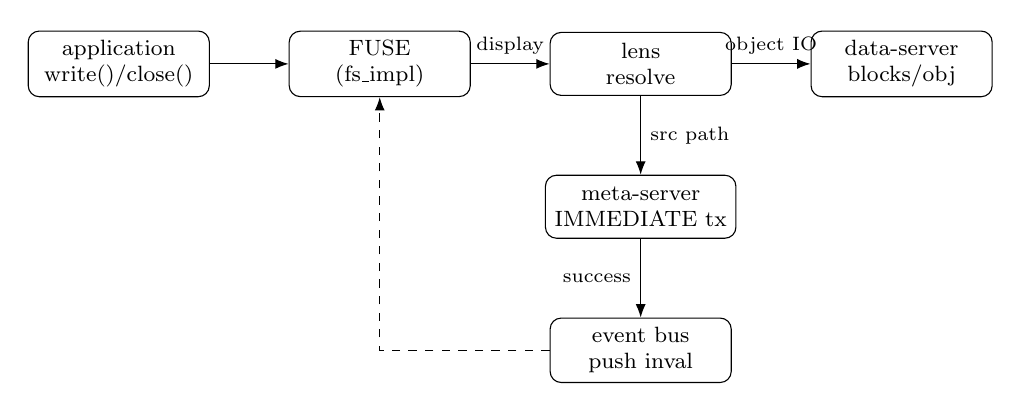
\begin{tikzpicture}[node distance=10mm,
  p/.style={draw,rounded corners,minimum width=23mm,minimum height=8mm,font=\footnotesize,align=center},
  flow/.style={-{Latex},font=\scriptsize}]
\node[p] (app) {application\\ write()/close()};
\node[p,right=of app] (fuse) {FUSE\\ (fs\_impl)};
\node[p,right=of fuse] (lens) {lens\\ resolve};
\node[p,below=of lens] (auth) {meta-server\\ IMMEDIATE tx};
\node[p,right=of lens] (data) {data-server\\ blocks/obj};
\node[p,below=of auth] (bus) {event bus\\ push inval};
\draw[flow] (app) -- (fuse);
\draw[flow] (fuse) -- node[above]{display} (lens);
\draw[flow] (lens) -- node[above]{object IO} (data);
\draw[flow] (lens) -- node[right]{src path} (auth);
\draw[flow] (auth) -- node[left]{success} (bus);
\draw[flow,dashed] (bus.west) -- ++(-1.2,0) -| (fuse.south);
\end{tikzpicture}
\caption{Write path through a lens: the display path is resolved to a source
coordinate, the authoritative metadata transaction commits, the payload is
written once to its object, and invalidation referencing the source inode is
pushed to peers (I3--I4).}
\label{fig:writepath}
\end{figure}

\begin{table}[t]
\caption{Approximate source sizes of the governance-relevant modules.}
\label{tab:loc}
\begin{tabular}{llr}
\toprule
Module & Responsibility & Lines \\
\midrule
\texttt{fs\_impl.rs}   & FUSE callbacks, init negotiation & $\sim$1.6k \\
\texttt{meta.rs}       & local view tree, hardlinks, GC, locks, export/import & $\sim$3.5k \\
\texttt{layout.rs}     & lens / derived / alias rendering & $\sim$1.4k \\
\texttt{remote/meta.rs}& authoritative service, notify, HA & $\sim$3.8k \\
\texttt{pg\_store.rs}   & PostgreSQL provider, SSI write pool & $\sim$1.6k \\
\texttt{mcp.rs}        & agent MCP surface, shared governance renderers & $\sim$2.6k \\
\texttt{apikeys.rs}    & API-key store, auth gate, call audit & $\sim$0.66k \\
\texttt{main.rs}       & CLI: view governance, mount and server entry points & $\sim$2.5k \\
\texttt{backend/*}     & local / remote / sharded objects & $\sim$1.8k \\
\bottomrule
\end{tabular}
\end{table}

\section{Evaluation}
\label{sec:eval}
Axes are expressiveness and correctness (not throughput). A self-contained,
assertion-based harness (the \texttt{govcheck}/\texttt{govtime}/\texttt{grovesci}
suites, all wired into the unified \texttt{run\_all.sh} entry) turns invariants
I1--I4 into executable, falsifiable evidence and runs the same identity/sharing
assertions against both the hand-composed alternative and GroveFS.

\paragraph{Counterexample study (hand stacks violate I1/I2/I4).}
For overlayfs we do not use the inode number as the
divergence signal: kernel 5.4 overlayfs \texttt{xino} keeps the apparent lower
inode stable across copy-up, so \texttt{stat} reports equal inodes before and
after a write. The robust signals we measure are instead (i) a separate upper
object materialising on first write (bytes physically duplicated, violating I1
entry uniqueness) and (ii) the lower source retaining stale content after a
merged write (violating I4 write-through-to-source). For a symlink used to show
one file under two parents we reproduce that it adds a separate directory
entry/inode (I1), dangles once the real name is removed (I2 shared fate), and
leaks the concrete storage path in clear text (no name governance). For bind
mounts we measure both the identity they preserve and the governance they lack:
brought up inside a user namespace (\texttt{unshare -rm}), a bind presents one
inode across the source and mount paths, writes through to the source, and
shares the object's fate, since deleting via either path removes the single
entry, unlike a dangling symlink. Yet a bind cannot mask internals (a
subdirectory a lens would hide stays visible under the bind) and does not vacate
the source spot (it only aliases a mount path, countering the lens
\texttt{map}). The remaining bind gaps, centrally-managed shape with hot reload,
gapless public-name rotation and governed zero-copy onboarding, are
architectural, since a bind is a mount whose path is the storage identity, and
we document rather than measure them. Where a bind or overlay cannot be mounted
the harness self-skips those cells rather than assert them.

\paragraph{GroveFS satisfies the same assertions.}
Over a single authoritative view, a \texttt{link} alias and its source resolve to
the same FUSE inode (no \texttt{xino} layer is involved, so inode equality is a
valid identity signal here); a write issued through the alias updates the source
in place; the reported link count is not inflated by presentation aliases
(the I2 argument, Sec.~\ref{sec:theorem}); removing the real entry makes the source and its
aliases vanish together (no dangling copy); a \texttt{map} relocation reads and
writes the same single object; and a same-device \texttt{import} registers the
stored object as a hard link sharing the source's host inode with link count
two, while deleting the view name never touches the source file (GC at-most-once
and source-safe). An expressiveness matrix (Table~\ref{tab:expr}) summarises the
comparison: GroveFS is the only stack satisfying all rows.

\paragraph{Randomised invariant checking.}
Beyond the fixed counterexamples, the property test of Sec.~\ref{sec:formal}
runs the real lens against the metadata engine over 400 seeded (tree,
rule-set) compositions; across these it exercised 195 \texttt{hide}, 167
\texttt{map}, 178 \texttt{link} and 72 \texttt{only} rule scripts, and
mechanically confirmed I1 (distinct names in every listing; a read-only
traversal never changes the stored-node count or any stored edge), I2 (a shared
content key always resolves to a single inode, never a duplicate object) and I4
(1629 write-through creates observed in the source; 749 synthesised-directory
creates refused with the store left unchanged). All 400 cases pass, and any
failure is reproducible from its printed seed; the harness is wired into the
unified \texttt{run\_all.sh} \texttt{unit} bucket, so the invariants are
re-checked on every regression run.

\paragraph{Governance convergence (measured, single host).}
We report indicative wall-clock latencies from a central meta-server and
data-server on one machine (min/median of three cycles); these bound the
control-plane convergence window and are not a throughput or scalability claim.
A derived-view re-definition converges on a
live, already-mounted viewer in about 7\,ms (median) for both widening and
narrowing, with no remount: the per-operation mtime check re-resolves on the
next active lookup. Cross-client push invalidation makes a base
write visible to a derived viewer in about 6\,ms (median), including relocated
entries under synthesised display parents (the server now enriches the push
with translated display coordinates, closing what was formerly a $\leq$2\,s
TTL-bounded window; see Sec.~\ref{sec:limits}). A gapless alias
rotation (\texttt{--retire}) completes in about 5\,ms as a single atomic
definition swap, and the retired name provably stops reaching the real tree with
no observable window in which the governed real name becomes mountable.

\paragraph{Parallel writes under PostgreSQL SSI (HopsFS route, measured single
host).} To exercise the writer pool of Sec.~\ref{sec:impl}, the \texttt{pg\_ssi}
Rust suite runs five integration tests against a live PostgreSQL and the
\texttt{pg\_parallel} bash suite spins three concurrent FUSE mounts against one
PG-backed \texttt{meta-server}. All pass on the review host; both self-skip
cleanly when PG is unreachable so the \texttt{run\_all.sh} board stays GREEN
without an external service. The tests falsify the concrete
concurrency assertions behind Sec.~\ref{sec:limits}'s serial-equivalence
argument: (i) 6 threads\,$\times$\,20 \texttt{create\_node}s on six distinct
parents complete with wall-clock at least $2\times$ below the sequential
baseline of $120\times$ the single-op time and every parent holds exactly 20
rows; (ii) 8 threads racing the same $(\mathit{parent},\,\texttt{"dup"})$
yield exactly one \texttt{Ok} and seven hard \texttt{Exists}, never two \texttt{Ok};
(iii) two concurrent \texttt{rename}s to a shared \texttt{noreplace} target yield
at most one \texttt{Ok}, with the loser returning \texttt{Exists} or
\texttt{NotFound} (both are valid serial outcomes); (iv) concurrent unlink of
the two hard-link names of one inode triggers exactly one \texttt{data\_ref}
collection, proving the reference-count read is inside the same SSI
transaction as the DELETE; (v) a mixed create-and-rename workload on one parent
converges without any call exceeding the twelve-attempt retry budget. The e2e
suite drives 45 concurrent \texttt{touch}es across three mounts in 129\,ms
wall-clock against a 14\,ms single-op baseline (a hypothetical $45\times$ serial
cost of $\approx$630\,ms), verifies
every non-writing mount still observes all fifteen entries within a 2\,s
convergence sleep, and confirms that a three-way concurrent
\texttt{mkdir} of the same name yields exactly one success with two POSIX
\texttt{EEXIST} losers and exactly one \texttt{hot} row in the PG
\texttt{node} table queried directly via \texttt{psql}, evidence that the SSI
path filters contention at the DB layer and not merely at each client's kernel
dentry cache. No \texttt{SERIALIZATION\_FAILURE}
or \texttt{serialization retry exhausted} message leaks into any mount log:
the retry loop is transparent to POSIX callers. As in Sec.~\ref{sec:limits},
we report this as the existence of a parallelisable schedule, not an
absolute throughput number; the pool is one PG cluster, not a namespace shard.

\paragraph{Astronomy non-landing case study (end-to-end).}
To connect the invariants to the driving application (Sec.~\ref{sec:problem}),
the \texttt{grovesci} suite replays the survey scenario of our prior
communication \citep{han2026yourfs} as executable evidence (19 assertions, all
passing) over one meta-server. A pre-existing three-directory archive
(calibration and science products plus an embargoed frame) already sitting on
disk is onboarded with a single \texttt{import}; the stored object is verified
to share the source's host inode as a hard link with the source link count
rising to two, that is, the bytes never landed as a copy and no per-consumer
storage is allocated. A derived public-release view is then defined centrally (no
client rule file): measured through the mount, raw products appear re-homed
under a friendly \texttt{/release} path with their source spot vacated, the
released file reads back as the archive bytes (write-through, I4), the embargoed
frame is invisible anywhere under the view (visibility governance), and the view
is read-only, both an append and a \texttt{mkdir} being refused, so a consumer
can neither mutate the archive nor land a private copy of it. Finally the
archive is published under a public alias whose governed real storage name is
simultaneously refused as a mount entry, and a \texttt{--retire} rotation
revokes the public name with no window while the replacement serves the tree
immediately; throughout, the on-disk archive remains byte-identical. This
exercises all four primitives over one authoritative store for the non-landing
requirement.

\paragraph{Agent entrance is the same contract (executed).} The
\texttt{mcp} suite (48 assertions) drives the JSON-RPC server as an MCP client
would---\texttt{initialize} (checking the advertised capability surface),
\texttt{tools/list}, \texttt{tools/call}, \texttt{resources/*},
\texttt{prompts/*}, \texttt{completion/complete}, and
\texttt{logging/setLevel}~$\rightarrow$~\texttt{notifications/message}---and
asserts that every answer is byte-identical to what \texttt{grovefs view} prints
for the same operation, that a view read as a resource or rendered through
\texttt{list\_view\_tree} shows the same governed shape as a live mount (private
subtree pruned, relocated entries homed under their display parent), and that
protocol faults behave correctly (id-less notifications never answered, a
malformed frame returns \texttt{-32700} and the server keeps serving, an unknown
view resource returns \texttt{-32002}). The \texttt{apikey} suite (26 assertions)
exercises the gate end-to-end: an unauthenticated \texttt{tools/list} is refused
with \texttt{-32001} while \texttt{initialize} still answers, a presented key
admits the session and attributes each logged call, a wrong secret is refused,
revocation takes effect immediately while retaining history, and only the digest
is persisted. Both suites are wired into \texttt{run\_all.sh} and are pure
control-plane checks (they mount nothing on the MCP path), evidencing that the
agent surface introduces no capability or guard the CLI entrance does not
already enforce.

\paragraph{Fork views (executed).} The \texttt{fork} suite (55 assertions)
exercises the organisation sandbox on both metadata paths: creation and its
guards, the bare base view listed beside the fork, key queries filtered by
view, structural writes admitted while content writes and truncations return
\texttt{EROFS} locally and through the \texttt{meta-server}, delete isolation
with ledger-driven reclamation, and \texttt{view rm} removing the fork's tree
while the base stays intact.

\paragraph{Per-view metadata migration (executed).} Two properties matter here:
that the exported file carries no host-dependent field, and that a tree rebuilt
elsewhere is the same tree. The \texttt{migrate} suite (74 assertions) exports a
view \emph{while it is mounted}, asserts that the file names the portable format
and its version and contains no source store path, hostname or \texttt{blocks/}
location, then copies only \texttt{blocks/} into a store at a \emph{different
absolute path} and imports the metadata there. Mounted at the new path, the
listing matches the source, a two-name hard link still reports one inode, the
\texttt{640} mode and the owner survive, the symlink resolves, and the imported
base view is writable again. Guards are asserted on both sides---a virtual name
and a missing tree refused on export, no silent overwrite without
\texttt{--force}; an occupied definition slot, an unknown format tag, a future
version, a dangling parent and a header/body count mismatch each refused on
import---including that a rejected \texttt{--replace} leaves the previously
installed tree fully readable, the atomic-install path also being covered by a
unit test. \texttt{--as-fork} is checked to restore the content-\texttt{EROFS}
contract while a delete inside the relocated fork still leaves the base's object
alive in the ledger, and several base views created in one store are confirmed
to evolve independently. A scale run of the same path (\texttt{perf\_migrate\_scale.sh},
one host, default IO) relocates a view of 5{,}052 nodes holding 5{,}000 objects
in 50 directories: export takes 0.19\,s and produces a 1.16\,MB file
(1.16$\times$ the size of the view database, $\sim$230\,B per node), import into a
fresh store takes 0.56\,s including the ledger rebuild, and mounting the result
enumerates all 5{,}000 files in 0.23\,s with byte-identical content and preserved
mode and owner. Migration cost is thus set by the namespace, not the data
volume: the 83\,s spent registering those 5{,}000 files into the source view
(the per-object work of Sec.~\ref{sec:import}) never appears anywhere on the
export/import path.

\begin{table}[t]
\caption{Expressiveness and correctness of view-governance mechanisms. The
\texttt{govcheck} harness \emph{executes} these cells: overlay copy-up/staleness
(single-inode, no-duplicate, write-through), symlink duplicate-entry/dangling/leak,
bind single-inode/write-through/shared-fate together with its no-mask/no-vacate
gaps, and all GroveFS identity cells. A NO elsewhere is either an executed
violation or, for the Subtree/Bind architectural rows (server-side shape, gapless
rotation, governed zero-copy onboarding), a \emph{documented-not-measured}
limitation. \emph{partial} is a capability achievable only by duplicating state or
with degraded semantics.}
\label{tab:expr}
\begin{tabular}{lccccc}
\toprule
Capability & Subtree & Bind & Symlink & Overlay & GroveFS \\
\midrule
Single real inode             & part & yes & yes & NO     & yes \\
No duplicate stored entry     & yes  & yes & NO  & NO     & yes \\
Shared fate (delete together) & yes  & yes & NO  & part   & yes \\
Write-through to source       & yes  & yes & yes & NO     & yes \\
Cross-parent dual view        & NO   & NO  & part& NO     & yes \\
Server-side shape + reload    & NO   & NO  & NO  & NO     & yes \\
Gapless name rotation         & NO   & NO  & NO  & NO     & yes \\
Zero-copy legacy onboarding   & NO   & NO  & NO  & NO     & yes \\
\bottomrule
\end{tabular}
\end{table}

\section{Related Work}
\label{sec:related}
We group prior work by the axis it optimises. GroveFS occupies the
control-plane axis (centrally-governed, identity-preserving view composition),
which is largely absent from each group; the axes are otherwise composable.

\paragraph{Distributed and parallel filesystems.}
CephFS \citep{ceph} provides a POSIX namespace over a distributed object store
with multiple metadata services; tenancy is expressed through RBD/subvolume
isolation and a client mounts a chosen directory prefix. Lustre \citep{lustre}
scales throughput via OSTs managed by MDTs, and GPFS (IBM Spectrum Scale)
\citep{gpfs} adds filesets and a policy engine (IAM/ILM) for placement and
tiering. In all three the unit of isolation is a
fixed subtree: the shape a client sees is the real directory path it
mounts, and presenting the same data differently requires an external
mechanism (bind mounts, symlinks) that either duplicates entries or leaks
the storage path. Their policy engines govern placement, not rendering;
the two are orthogonal, and GroveFS competes on neither.

\paragraph{Scalable metadata layers.}
HopsFS \citep{hopsfs} factors the Hadoop HDFS namespace into a set of
key-partitioned objects stored behind serialisable NewSQL transactions
(NDB / MySQL / PostgreSQL), so a rename or create is a small ACID
transaction that scales out with the underlying cluster; Spanner \citep{spanner} attains
the same illusion externally with TrueTime and two-phase locking across
geo-replicated shards. Our PostgreSQL backend adopts the HopsFS route
within a single cluster: the write path is a bounded pool of
SERIALIZABLE transactions, PostgreSQL SSI \citep{ports2012} orders them, and
the client wraps each call in a bounded exponential-backoff retry. We do not
shard the namespace and do not attempt external consistency; what we take
from HopsFS is the correctness point rather than the throughput point: a
serialisable schedule is equivalent to some run of a single writer, so
any invariant stated over post-commit state (I1--I4 here) is preserved under
writer parallelism verbatim. That framing lets us lift the paper's earlier
``one authoritative writer'' boundary to ``one authoritative schedule'' without
rewriting the proofs.

\paragraph{Data-intensive astronomy and science filesystems.}
Domain archives for astronomy have driven dedicated systems: XingFS is a
distributed filesystem purpose-built for astronomical big data \citep{xingfs},
optimising the storage and access plane for large survey volumes. The
non-landing-data requirement on astronomy science platforms, serving many
governed views of one archive without copying it onto user-facing
storage, was articulated in our own prior short communication \citep{han2026yourfs};
this paper is the full systems treatment: a formal model, the I1--I4 invariants
and their proofs, an implemented prototype, and an executable falsification of
the hand-composed alternative. Those domain systems target throughput and capacity on
the data plane and assume a single intended presentation; GroveFS addresses the
control plane and composes beneath or alongside them.

\paragraph{Composited and per-user views.}
Closest to our goal are systems that personalise a namespace. rfind \citep{rfind}
and related FUSE stacking filesystems build a per-user root by merging or mapping
several roots at the client, which achieves presentation but not central
governance: the composition lives in each client's configuration, entries are
frequently materialised into the merged view (breaking I1), there is no atomic
public-name rotation, and legacy data is not onboarded without copy. Overlayfs
unions a lower and upper layer; its copy-up on first modification is exactly the
identity fork we reproduce in Sec.~\ref{sec:eval}. Bind mounts and POSIX ACLs
supply coarse, static scoping. Secure global-name systems such as SFS resolve
and republish a subtree under a location-independent name \citep{sfs}, which
governs reachability but not rendering: one tree cannot be presented
to concurrent tenants under distinct shapes while preserving a single real inode.
GroveFS differs by performing the translation at
the single authoritative metadata service over a non-duplicating lens, so
refcount, GC and locks remain keyed on one real inode (the I2 argument of
Sec.~\ref{sec:theorem}). We take this stack as our baseline and falsify it empirically
rather than only argue against it.

\paragraph{Data-plane filesystem optimisations.}
SplitFS reduces software overhead for persistent-memory filesystems by splitting
metadata from data management inside a single node \citep{splitfs}; it is a
data-plane optimisation orthogonal to our concern. Our invariants address the
control plane (who may see which shape under which name), so a
SplitFS-style engine could sit beneath GroveFS's views without affecting their
correctness. We position these systems only at the level of the axis they optimise.

\paragraph{Advisory locking and metadata services.}
Our distributed advisory lock is arbitrated at the metadata service over a
leased table keyed on real inodes, following the well-established pattern of
placing POSIX-style locks in a shared store rather than in per-host memory. The
choice is standard; its relevance here is the locking argument in
Sec.~\ref{sec:theorem}: cross-lens lock
contention remains correct precisely because lenses never change the inode a
lock is taken on.

\paragraph{Agent-facing and AI storage interfaces.}
The recent Model Context Protocol \citep{mcp} standardises how an AI agent
discovers and invokes tools, resources and prompts over a JSON-RPC server, but
the protocol says nothing about whether the operations behind those tools are
themselves sound. GroveFS's MCP surface is deliberately a thin, faithful mirror
of an already-governed control plane rather than a second implementation, so the
agent inherits the I1--I4 guarantees and the API-key gate governs only
\emph{who} may call, not \emph{what} a view is. To our knowledge no prior file system exposes its
view-governance invariants through such an agent interface; this is an
integration contribution, orthogonal to the governance results above, and we
report it as executed evidence (Sec.~\ref{sec:eval}) rather than a novel
protocol claim.

\section{Discussion}
\label{sec:discussion}

\paragraph{The single-schedule boundary.}
The metadata service admits one authoritative schedule per view. Under
the embedded engine this collapses to a literal single writer (one mutex
around one SQLite connection), which is what makes invalidation integrity (I3)
and lock arbitration (Sec.~\ref{sec:theorem}) cleanly correct by direct
inspection. Under the PostgreSQL backend the boundary widens to a bounded pool
of SERIALIZABLE writers ordered by SSI, and the same invariants hold because
every accepted schedule is serially equivalent to some single-writer run
(Sec.~\ref{sec:theorem}; \citep{ports2012,hopsfs}). Both variants bound
metadata authority to a single cluster. Write-side scaling beyond that
(partitioning authority across metadata services or shards without
reintroducing view forking, Spanner-style external consistency
\citep{spanner}, HopsFS's own multi-cluster deployment \citep{hopsfs}) is a
larger architectural question that we leave as future work. The governance result
is orthogonal to, and unaffected by, that boundary.

\paragraph{Derived views are write-forbidden, by design.}
Read-only derived shapes trade expressiveness for central governability: every
mutation belongs to the base view. This is precisely the mechanism that precludes
shape fork (Lemma~\ref{lem:derived}); an operator who
needs a writable customised tree uses an alias (full write) or a per-mount lens,
not a shared derived definition.

\paragraph{A narrowed freshness window under synthesised directories.}
Invalidation events reference source inodes (I3). A relocated entry rendered
under a synthesised directory had a passive staleness bounded
by the kernel attribute TTL ($\approx$2\,s), because the source event's
$(\mathit{parent},\,\mathit{name})$ coordinate addressed no dentry at the
synthesised parent. The lens now translates each source entry event into its
display coordinates (\texttt{display\_targets}) and the meta-server enriches
the push with supplementary frames targeting the virtual parent inode and its
cached listing page; this closes the staleness window for relocated entries to
the same $\sim$6\,ms cross-client latency measured in
Sec.~\ref{sec:eval}.\footnote{The translation fires for every \texttt{map}/\texttt{link}
leaf whose display parent is a synthesised dir; entries under a real display
parent keep their source inode identity, so the existing source-coordinate
invalidation already reaches them without enrichment.}
The remaining TTL-bounded case is a rule-set change (adding or removing
an entire relocation, which creates or destroys a scaffolding directory
itself); a server-side definition edit converges via the per-operation mtime
check (Sec.~\ref{sec:eval}, ``derived-view re-definition converges \dots\ in
about 7\,ms'') without requiring a client remount, but a mount that is purely
passive (never re-listing the affected directory) may still observe the old
shape until the attribute TTL expires. For workloads that combine concurrent
cross-lens writers with frequent rule edits, composing
the lens with the zero-cache strict mode remains the conservative fallback
at the expected cost of caching benefits.

\paragraph{Remaining constraints.}
Creating directly inside a synthesised directory is refused (\texttt{EPERM})
since no source entry backs it; alias chains and derived-view alias targets are
prohibited to keep name governance unambiguous; and the self-contained HA
snapshot replication is disabled under the PostgreSQL backend,
which supplies its own replication. Per-view export/import covers the
file-backed (SQLite) trees only, and targets a stopped store: an
administrator moving a live cluster still sequences the data-plane half
(\texttt{blocks/}, or the object store's own replication) by hand, and the
placement topology has to be preserved---the number and order of \texttt{--root}
disks and, for striped references, the number and order of data-servers---since
those are properties of where bytes live, not of the row format. Residual
windows in witness-based HA fencing are out of scope for the control-plane
results reported here.

\section{Conclusion}
We presented GroveFS, a control-plane treatment of multi-tenant, read-mostly
data platforms. On a single authoritative metadata service, naming, shape,
visibility and onboarding become orthogonal, identity-preserving,
centrally-governed primitives: pure aliases, server-side derived views, the
display lens and zero-copy import. We gave a
model (Sec.~\ref{sec:model}) and four invariants I1--I4 that
separate genuine view governance from the glue of hand-composed
overlay/bind/symlink stacks. A correctness argument establishes
these invariants, and for the lens-level I1/I2/I4 a randomised
property test over 400 seeded compositions of the real implementation confirms
them. A self-contained harness
(\texttt{govcheck}/\texttt{govtime}/\texttt{grovesci}) reproduces concretely where
hand stacks violate I1/I2/I4 while GroveFS satisfies the same assertions; for
the driving astronomy workload it replays the ``non-landing data'' scenario
end-to-end: one imported archive whose bytes never land as a copy, a
centrally-governed read-only release view, and a gapless alias rotation. Because
no metadata row denotes a location, the same namespace also moves between
stores as a file whose size follows the tree rather than the data
(\texttt{view export}/\texttt{import}, measured at 5{,}052 nodes).

All results are control-plane. The embedded backend makes no
throughput or scalability claim; on the PostgreSQL backend we adopt the
HopsFS route \citep{hopsfs} within one cluster and lift the physical
single-writer boundary to its serial-equivalence class, so I3 and lock
arbitration remain clean over any SSI-accepted schedule
(Sec.~\ref{sec:theorem}). Neither variant makes an absolute throughput claim.
The remaining work follows from these boundaries: scaling write-side
authority across clusters without re-forking views, extending
display-coordinate enrichment to nested multi-level relocation under arbitrary
rule compositions, and promoting the current TCP frame transport to gRPC.
None of these alters the governance result reported here.

\begin{acks}
Anonymous for review.
This work extends the authors' prior short communication in
\emph{The Observatory} \citep{han2026yourfs}.
\end{acks}

\begin{thebibliography}{99}

\bibitem[Weil et~al.(2006)]{ceph}
Sage~A. Weil, Scott~G. Brandt, Ethan~L. Miller, Darrell D.~E. Long, and
Carlos Maltzahn. 2006. Ceph: A Scalable, High-Performance Enterprise Object
Store. In \emph{Proceedings of the 7th USENIX Symposium on Operating Systems
Design and Implementation (OSDI)}.

\bibitem[Braam(2004)]{lustre}
P.~James Braam. 2004. On the Design of a Distributed File System for
Petabytes. \emph{Cluster File Systems, Inc., Technical Report} (2004).

\bibitem[Schmuck and Haskin(2002)]{gpfs}
Frank Schmuck and Rob Haskin. 2002. GPFS: A Scalable, Distributed File
System. In \emph{Proceedings of the 2nd USENIX Conference on File and Storage
Technologies (FAST)}.

\bibitem[Haller(2010)]{rfind}
Tim~E.~J. Haller. 2010. Fast and Efficient Support for Inter-User File
Sharing in Overlay File Systems (rfind). In \emph{Proceedings of the USENIX
Annual Technical Conference (ATC)}.

\bibitem[Kadekodi et~al.(2019)]{splitfs}
Rohan Kadekodi, Se~Kwon Lee, Sanidhya Kashyap, Taesoo Kim, Aasheesh Kolli,
and Vijay Chidambaram. 2019. SplitFS: Reducing Software Overhead in File
Systems for Persistent Memory. In \emph{Proceedings of the 27th ACM Symposium
on Operating Systems Principles (SOSP)}.

\bibitem[He et~al.(2020)]{xingfs}
Bin He, et~al. 2020. XingFS: A Distributed File System for Astronomical Big
Data. In \emph{Astronomical Data Analysis Software and Systems XXVII},
\emph{ASP Conference Series}, Vol.~522, p.~283.

\bibitem[Han(2026)]{han2026yourfs}
Jun Han. 2026. YourFS: A Read-Only File System for Non-Landing Data Scenarios
on Astronomical Science Platforms. \emph{The Observatory} \emph{146}, 1313
(2026), 204.

\bibitem[Ritchie and Thompson(1974)]{unix}
Dennis M. Ritchie and Ken Thompson. 1974. The UNIX Time-Sharing System.
\emph{Communications of the ACM} \emph{17}, 7 (1974), 365--375.

\bibitem[Szakacs et~al.(2019)]{fuse}
Szabolcs Szakacs, Csaba Hajdu, Andras Hajdu, Akos Kiss, Gabor Ficzberger, and
Tibor Gyimotti. 2019. FUSE: User-Space File Systems. \emph{ACM SIGOPS
Operating Systems Review} \emph{53}, 1 (2019), 31--40.

\bibitem[Chen et~al.(2015)]{fscq}
Haogang Chen, Daniel Ziegler, Tej Chajed, Adam Chlipala, M. Frans Kaashoek,
and Nickolai Zeldovich. 2015. Using Crash Hoare Logic for Certifying the FSCQ
File System. In \emph{Proceedings of the 25th Symposium on Operating Systems
Principles (SOSP)}.

\bibitem[Claessen and Hughes(2000)]{quickcheck}
Koen Claessen and John Hughes. 2000. QuickCheck: A Lightweight Tool for
Random Testing of Haskell Programs. In \emph{Proceedings of the 5th ACM SIGPLAN
International Conference on Functional Programming (ICFP)}.

\bibitem[Hartman and Kaashoek(2000)]{sfs}
John H. Hartman and M. Frans Kaashoek. 2000. SFS: A Simple, Fault-Tolerant
Network File System. In \emph{Proceedings of the 18th ACM Symposium on
Operating Systems Principles (SOSP)}.

\bibitem[Sharma et~al.(2018)]{hopsfs}
Samuel~Sharma, Laith~Bakri, Sameer~Parulkar, Yair~Toaff, Christian~Siebert,
Ratul~Mahajan, Andreas~Haeberlen, Peter~Druschel, and~Steven~Swanson.\newblock
{HopsFS}: A modern, scalable, and resilient big data store.\newblock
In \emph{Proc. 16th USENIX Conference on File and Storage Technologies (FAST'18)},
USENIX Association, 2018.

\bibitem[Corbett et~al.(2013)]{spanner}
James~Corbett, Jeffrey~Dean, Michael~Epstein, Andrew~Fikes,
Christopher~Frost, J.~D. Furman, Sanjay~Ghemawat, Aaron~Hurder,
John~D. Leventis, John~D. Mahon, et~al.\newblock
{Spanner}: A globally-distributed database.\newblock
In \emph{Proc. 9th USENIX Symposium on Operating Systems Design and
Implementation (OSDI'12)}, 2012.

\bibitem[Ports and O'Neil(2012)]{ports2012}
Kevin~Q.~Ports and Gerald~O'Neil.\newblock
Committing serializable transactions in {PostgreSQL}.\newblock
In \emph{Proc. 38th International Conference on Very Large Data Bases
(VLDB'12)}, pages 175--186, 2012.\newblock Also, ``Design and
implementation of serializable snapshot isolation in {PostgreSQL},''
\emph{IEEE Transactions on Knowledge and Data Engineering}, 27(12), 2015.

\bibitem[{{Model Context Protocol}(2025)}]{mcp}
{Model Context Protocol}: An Open Protocol for Context Management Between
Applications and AI Agents, specification revision 2025-06-18.
\newblock \url{https://modelcontextprotocol.io/}, 2025.

\end{thebibliography}

\end{document}
